\documentclass[12pt,a4paper]{article}
\usepackage[utf8]{inputenc}
\usepackage[english]{babel}

\usepackage{amsmath}
\usepackage{amsfonts}
\usepackage{amssymb}

\usepackage{graphicx}
\usepackage{lmodern}
\usepackage{tikz}
\usepackage{titlesec}
\usepackage{environ}
\usepackage{xcolor}
\usepackage{fancyhdr}
\usepackage[colorlinks = true, linkcolor = black]{hyperref}
\usepackage{xparse}
\usepackage{enumitem}
\usepackage{comment}

\usepackage[left=2cm,right=2cm,top=2cm,bottom=2cm]{geometry}
\usepackage{multicol}
\usepackage[indent=0pt]{parskip}

\newcommand{\spaceP}{\vspace*{0.5cm}}
\newcommand{\Span}{\mathrm{Span}\,}
\newcommand{\range}{\mathrm{range}\,}
\newcommand{\ra}{\rightarrow}

%% Redefining sections
\newcommand{\sectionformat}[1]{%
    \begin{tikzpicture}[baseline=(title.base)]
        \node[rectangle, draw] (title) {#1};
    \end{tikzpicture}
    
    \noindent\hrulefill
}

% default values copied from titlesec documentation page 23
% parameters of \titleformat command are explained on page 4
\titleformat%
    {\section}% <command> is the sectioning command to be redefined, i. e., \part, \chapter, \section, \subsection, \subsubsection, \paragraph or \subparagraph.
    {\normalfont\large\scshape}% <format>
    {}% <label> the number
    {0em}% <sep> length. horizontal separation between label and title body
    {\centering\sectionformat}% code preceding the title body  (title body is taken as argument)

%% Set counters for sections to none
\setcounter{secnumdepth}{0}

%% Set the footer/headers
\pagestyle{fancy}
\fancyhf{}
\renewcommand{\headrulewidth}{0pt}
\renewcommand{\footrulewidth}{2pt}
\lfoot{P.-O. Paris{\'e}}
\cfoot{MATH 302}
\rfoot{Page \thepage}

%% Defining example environment
\newcounter{example}[section]
\NewEnviron{example}%
	{%
	\noindent\refstepcounter{example}\fcolorbox{gray!40}{gray!40}{\textsc{\textcolor{red}{Example~\theexample.}}}%
	%\fcolorbox{black}{white}%
		{  %\parbox{0.95\textwidth}%
			{
			\BODY
			}%
		}%
	}

% Theorem environment
\NewEnviron{theorem}%
	{%
	\noindent\refstepcounter{example}\fcolorbox{gray!40}{gray!40}{\textsc{\textcolor{blue}{Theorem~\theexample.}}}%
	%\fcolorbox{black}{white}%
		{  %\parbox{0.95\textwidth}%
			{
			\BODY
			}%
		}%
	}

\NewEnviron{notes}%
	{%
	\noindent \fcolorbox{gray!40}{gray!40}{\textsc{\textcolor{blue}{Solution.}}}%
	%\fcolorbox{black}{white}%
		{  %\parbox{0.95\textwidth}%
			{
			\textcolor{blue}{%
			\BODY
			}
			}%
		}%
	}
%%% Ignorer les notes
\excludecomment{notes}

%%%%
\begin{document}
\thispagestyle{empty}

\begin{center}
\vspace*{2.5cm}

{\Huge \textsc{Math 241}}

\vspace*{2cm}

{\LARGE \textsc{Chapter 2}} 

\vspace*{0.75cm}

\noindent\textsc{Section 2.7: Rates of Change}

\vspace*{0.75cm}

\tableofcontents

\vfill

\noindent \textsc{Created by: Pierre-Olivier Paris{\'e}} \\
\textsc{Fall 2022}
\end{center}

\newpage

\section{Rate of Change and Derivative}
Let $y = f(x)$ be a function.

\begin{multicols}{2}
\begin{itemize}
\item If $x$ goes from $x_1$ to $x_2$, then the change in $x$ is
	\begin{align*}
	\Delta x = x_2 - x_1 .
	\end{align*}
\item When $x$ changes from $x_1$ to $x_2$, then $y$ changes from $f(x_1)$ to $f(x_2)$ and the change in $y$ is
	\begin{align*}
	\Delta y = y_2 - y_1 = f(x_2) - f(x_1) .
	\end{align*}
\item The \textbf{average rate of change} at $x_1$ is therefore $\displaystyle \frac{\Delta y}{\Delta x}$.
\item The \textbf{instanteneous rate of change} at $x_1$ is
	\begin{align*}
	\frac{dy}{dx} = \lim_{\Delta x \ra 0} \frac{\Delta y}{\Delta x} .
	\end{align*}
\end{itemize}

\begin{center}
\includegraphics[scale=0.25]{section2-7_fig_1.png}
\url{https://www.desmos.com/calculator/ajsf8ggdwy}
\end{center}
\end{multicols}

\underline{Remark:} The name of the variables may be different. We can use the variables $x$, $t$ (or other letters) for the independent variable and $y$, $s$ (or other letters) for the dependent variable.

\vspace*{16pt}

\begin{example}
The position $s$ of an object is given by the function $s = f(t) = t^2$
	\begin{enumerate}
	\item[a)] Compute the average rate of change at $t_1 = 1$ if $t_1 = 1$ and $t_2 = 2$.
	\item[b)] Compute the instanteneous rate of change at $t_1 = 1$. 
	\end{enumerate}
\end{example}

\vfill

\underline{Remarks:} Let the position $s$ of an object be given by $s = f(t)$ where $f$ is a function of time $t$.
	\begin{itemize}
	\item The average velocity at $x_1$ is the average rate of change in $s$.
	\item The instanteneous velocity at $x_1$ is the instanteneous rate of change at $x_1$.
	\end{itemize}

\newpage

\section{Rates of Change in Physics}

	\subsection{Linear Density}
	Consider a rod.
	
	\vspace*{16pt}
	
	\begin{center}
		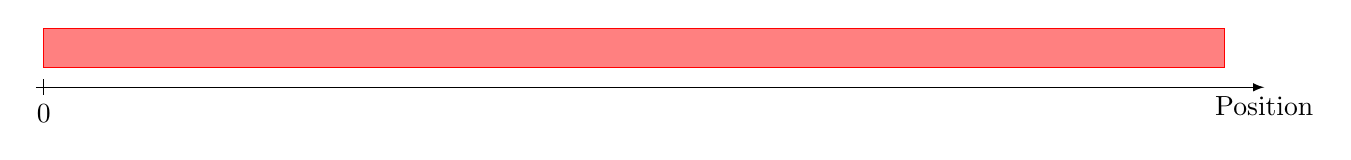
\begin{tikzpicture}
		\draw[red, fill=red!50] (0, 0) -- (15, 0) -- (15, 0.5) -- (0, 0.5) -- (0, 0);
		\draw[black, ->, >=latex] (-0.1, -0.25) -- (15.5, -0.25)node[below]{Position};
		\draw[black] (0, -0.15) -- (0, -0.35)node[below]{$0$};
		\end{tikzpicture}
	\end{center}
	
	\vspace*{16pt}
		
		\begin{itemize}
		\item The position on the rod from the extremity $0$ is given by $x$.
		\item The mass of the part of the rod from $0$ to $x$ is given by
			\begin{align*}
			m = f(x) .
			\end{align*}
		\end{itemize}
		
	\underline{Question:} How is the mass distributed along the rod?
	
	\begin{itemize}
	\item The \textbf{average linear density} between $x_1$ and $x_2$ is the average rate of change in the mass between $x_1$ and $x_2$.
	\item The \textbf{linear density} at $x_1$ is the instanteneous rate of change in the mass at $x_1$.
	\end{itemize}
	
	\vspace*{16pt}
	
	\begin{example}
	A rod as in the figure above has a mass $m$ given by $f(x) = x^3$.
		\begin{enumerate}
		\item[a)] Find the average linear density between $x_1 = 1$ and $x_2 = 2$.
		\item[b)] Find the linear density at $x_1 = 1$.
		\end{enumerate}
	\end{example}
	
	
\newpage

\section{Rate of Change and Epidemics}
Suppose there is a virus spreading in a population. We are interested in describing:
	\begin{itemize}
	\item The rate at which the virus spreads from one individual to another at a specific moment in time
	\item If we know the quantity of infected individuals, denoted by $Q(t)$.
	\end{itemize}
	
In this case, the rate at which the virus spreads between two days, day $t_1$ and $t_2$ respectively, is given by the average rate of change in $Q$:
	\begin{align*}
	\frac{\Delta Q}{\Delta t} .
	\end{align*}

Therefore, the rate at which the virus spreads at day $t_1$ is given by the instantaneous rate of change (when $\Delta t \ra 0$):
	\begin{align*}
	\frac{dQ}{dt} \text{ !}
	\end{align*}
	
\vspace*{16pt}
	
\begin{example}
Suppose a virus is spreading in the population of deers on Moloka'i. Suppose the number of infected deer at day $t$ is given by $Q(t) = (50/\pi ) \sin (\pi t) + 60$. Let $t = 0$ be the first day we observed the presence of the virus and the model is valid up to $t = 5$.
	\begin{enumerate}
	\item[a)] Find at which rate the virus spreads in the population at day $t = 3$.
	\item[b)] Estimates the number of deers infected at day $t = 6$.
	\end{enumerate}
\end{example}

\end{document}